%!TEX root = main.tex

\chapter{Analyse kohärenter Konstruktionen mit TAG-Varianten} \label{sec-kohaerenz-tag}

In Kapitel \ref{sec-valenz-tag} wurde die derivationelle Unzulänglichkeit des TAG-Formalismus bei der Bewältigung bestimmter Diskontinuitätsmuster\is{Diskontinuität}, die im Zusammenhang mit kohärenten Konstruktionen\is{kohärente Konstruktion} auf"|treten, deutlich. In diesem Kapitel gilt es, die bisherigen Anstrengungen darzustellen, den TAG-Formalismus ma\ss voll, d.\,h.\ im Rahmen der schwachen Kontextsensitivität\is{schwache Kontextsensitivität}, zu erweitern und mit der nötigen Ausdrucksstärke auszustatten. Wir werden sehen, dass all diese TAG"=Erweiterungen bestimmte Nachteile mit sich bringen und damit eine Bresche besteht, in die die von mir entwickelte TAG-Erweiterung, \isi{TT-MCTAG}, springen kann. TT-MCTAG wird im nächsten Kapitel ausführlich behandelt. 

Die Diskontinuitätsphänomene bei kohärenten Konstruktionen haben natürlich auch in anderen Syntax-Frameworks, die ebenfalls unter dem Einfluss der Idealisierung der Kontinuität stehen, eine reichhaltige Forschungsliteratur provoziert. Um den Horizont etwas zu erweitern und die grundsätzliche Ähnlichkeit der Syntax-Frameworks bei der Behandlung solcher Diskontinuitätsphänomene zu zeigen, wird im ersten Abschnitt zunächst eine allgemeine Taxonomie unterschiedlicher Modellierungsstrategien entwickelt. In Abschnitt \ref{sec-tag-varianten} folgt dann die Darstellung und Einordnung der bislang vorgeschlagenen TAG-Erweiterungen.  

\section{Modellierungsstrategien} \label{sec-ttmctag-modellierungsstrategien}

In dieser Arbeit wird Kohärenzmodellierung vom Standpunkt der \isi{Valenzrahmenrealisierung} aus betrachtet und danach richtet sich auch die Taxonomie der Modellierungsstrategien, die in Abbildung~\ref{fig-kohaerenz-strategien} dargestellt ist. Die Idealisierung der Kontinuität\is{Idealisierung!der Kontinuität} bei der Valenzrealisierung besagt, dass der Valenzrahmen als kontinuierlicher String realisiert wird (vgl.\ Abschnitt~\ref{sec-strukturfrage}). Dementsprechend erhält in einer Vielzahl von Modellierungsansätzen die kontinuierliche Valenzrahmenrealisierung einen primären Status, dem gegenüber die diskontinuierliche Valenzrahmenrealisierung nachgeordnet ist und nur durch zusätzliche Mechanismen oder Ableitungsschritte erfasst werden kann. In Abbildung \ref{fig-kohaerenz-strategien} fallen darunter die Modellierungsstrategien mit \isi{Bewegung} und \isi{Valenzvereinigung}. Ganz anders verhalten sich solche Modellierungsansätze, die Diskontinuität direkt repräsentieren.\footnote{Die Taxonomie in \citet[10ff]{Wurmbrand:01} hat nur die kontinuierliche Valenzrealisierung im Blick. Dort wird zwischen "`bi-clausal approaches"' ($\approx$ Bewegung) und "`mono-clausal approaches"' ($\approx$ Valenzvereinigung) unterschieden. An diese Taxonomie hält sich auch \citet[21]{Grosse:05}, nennt diese Klassen aber "`derivationelle Ansätze"' und "`basisgenerierte Ansätze"'. Siehe \cite{Wurmbrand:01} für eine umfassendere Literaturübersicht über Ansätze innerhalb der Generativen Grammatik\is{Generative Grammatik}.}

\begin{figure}
\centering
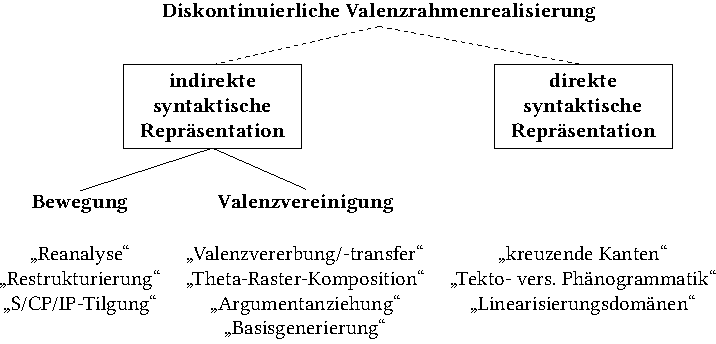
\includegraphics{graphics/abb61.pdf}
\caption{\label{fig-kohaerenz-strategien}Taxonomie der Diskontinuitätsmodellierung}
\end{figure}


\subsection{Bewegung}\is{Bewegung|(}

Bewegungsansätze leiten kohärente Strukturen aus inkohärenten Strukturen ab. \isi{Diskontinuität} ist also derivationell abhängig von Kontinuität. Dieser Prozess kann in Anlehnung an \citet[(1)]{Evers:75} so schematisiert werden wie in Abbildung \ref{fig-ttmctag-kohaerenz-1}.\footnote{Bei \citet[(1)]{Evers:75} sind die Terminale nicht indiziert. Da er die Wortstellung des Niederländischen im Blick hat, also {\it NP$_1$ NP$_2$ V$_1$ V$_2$}, beschränkt er sich in seiner Schemadarstellung auf die S-Tilgung ("`S-Pruning"') und V-Bewegung ("`V-Raising"').} Ausgangspunkt ist ein inkohärentes Satzgefüge mit eingebetteten S-Baum, aus dem in einem ersten Schritt mittels V-Bewegung ein \isi{Verbalkomplex} gebildet und der S-Knoten getilgt wird. In einem zweiten Schritt erfolgt die NP-Bewegung, so dass der diskontinuierlich indizierte Terminalstring {\it NP$_2$ NP$_1$ V$_2$ V$_1$} resultiert.  

\begin{figure}
\centering
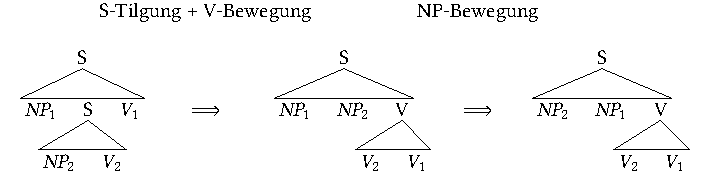
\includegraphics{graphics/abb62.pdf}
\caption{\label{fig-ttmctag-kohaerenz-1}Bewegungsstrategie nach \citet[(1a), (1b)]{Evers:75}}
\end{figure}

Der erste Schritt, der in der Literatur oft als \isi{Reanalyse} bezeichnet wird (\citealt{Haegeman:Riemsdijk:86}; \citealt[Kapitel~12]{Stechow:Sternefeld:88}; \citealt{Stechow:90}), schafft durch die S-Tilgung erst die Voraussetzung für die Möglichkeit, {\it NP$_1$} und {\it NP$_2$} zu scrambeln, da {\it NP$_2$} gemä\ss\ der üblichen Inselbeschränkungen nicht aus dem eingebetteten S-Baum (bzw.\ CP-Baum) herausbewegt werden kann. Darin wird der grundsätzliche Widerspruch deutlich, bei der Generierung diskontinuierlicher Strukturen von bi-sententialen Strukturen auszugehen, deren Wesensmerkmal gerade die Verhinderung von Diskontinuität ist. Funktionell analoge Mechanismen zur S-Tilgung, die diesen Widerspruch aufzulösen versuchen, finden sich also in allen Bewegunsansätzen der Generativen Grammatik\is{Generative Grammatik}, auch in denen, die nur Bewegung verwenden. Als Beispiele dafür seien \cite{Grewendorf:Sabel:94} und \cite{Sabel:96} genannt, wo CPs durch bestimmte Prozesse bewegungsdurchlässig oder "`transparent"' gemacht werden.\footnote{\citet[102]{Jacobs:92} beklagt aber, dass die Reanalyse eine "`unschöne"', "`weil prinzipienverletzende und strukturzerstörende"' Transformation sei. Ähnlich äu\ss ert sich \cite[257]{Haider:93}:
\begin{quote}
Im übrigen ist die Annahme von Reanalyse kontraproduktiv: Sie lä\ss t genau die Teil der Struktur verschwinden, deren Vorhandensein die beobachteten Phänomene verhindern würde, ohne da\ss\ es eine unabhängig motivierte Theorie für Reanalyseprozesse gäbe, aus der die Eigenschaften herleitbar wären.
\end{quote}
Haider hebt au\ss erdem hervor, dass die \isi{Reanalyse} nicht ohne Weiteres mit dem Fernpassiv\is{Passiv!Fern-} zurecht kommt \citep[254]{Haider:93}. Dass man durchaus das Fernpassiv in Bewegungsansätzen ohne Tilgung modellieren kann, zeigt \citet[204ff]{Sabel:96}.}   
\is{Bewegung|)}

\subsection{Valenzvereinigung} \label{sec:valenzvereinigung}\is{Valenzvereinigung|(}

Bei Ansätzen mit Valenzvereinigung werden die Valenzrahmen kohärent konstruierter Verben in einen gemeinsamen Valenzrahmen zusammengefasst, so dass das mittlere und das rechte Strukturschema in Abbildung \ref{fig-ttmctag-kohaerenz-1} direkt generiert werden können. Vom zusammengefassten Valenzrahmen aus betrachtet erfolgt die Valenzrahmenrealisierung also immer kontinuierlich, sei es mit oder ohne zusätzliche Bewegungstransformation. Im Rahmen der Generativen Grammatik\is{Generative Grammatik} haben einen Valenzvereinigungsansatz beispielsweise \cite{Jacobs:92} ("`Valenzvererbung"'), \citet[Abschnitt~9.6.2.2]{Haider:93}, \cite{Wurmbrand:01} und \citet[Kapitel~5]{Sternefeld:06} ("`Theta-Raster-Komposition"') ausgearbeitet. Doch dieser Ansatz findet sich auch schon in älteren Arbeiten zur \is{Kategorialgrammatik} \citep{Geach:70,Steedman:85} und GPSG\is{Generalized Phrase Structure Grammar (GPSG)} \citep{Johnson:86}. Nicht zuletzt gibt es eine Fülle von Arbeiten im Rahmen der HPSG\is{Head-driven Phrase Structure Grammar (HPSG)}, die auf Valenzvereinigung zurückgreifen, z.\,B.\ \cite{Hinrichs:Nakazawa:89,Hinrichs:Nakazawa:94} ("`argument raising"'), \cite{Nerbonne:94}, \cite{Pollard:96}, \cite{Meurers:99}, Müller (\citeyear[Kapitel~17--18]{Mueller:99}; \citeyear[Chapter~2]{Mueller:02}; \citeyear{Mueller:05}; \citeyear{Mueller:09}).\footnote{Wiewohl alle diese Arbeiten Valenzvereinigungsansätze darstellen, können sie sich doch in anderen Aspekten beträchtlich voneinander unterscheiden, etwa in der Frage, ob Verbbewegung\is{Bewegung} implementiert wird oder nicht. Siehe \cite{Meurers:99b} und \cite{Mueller:05} für eine Übersicht und weitere Literatur.}
\is{Valenzvereinigung|)}


\subsection{Direkte diskontinuierliche Valenzrealisierung} \label{sec-kohaerenz-strategien-direkt}

Die direkte Repräsentation der diskontinuierlichen Valenzrealisierung im indizierten String {\it NP$_2$ NP$_1$ V$_2$ V$_1$} bewerkstelligt etwa die Phrasenstruktur in Abbildung~\ref{fig-ttmctag-kohaerenz-2} mit einer kreuzenden Kante\is{kreuzende Kante}. Zweifelsohne kann eine kanonische CFG\is{kontextfreie Grammatik} solche Strukturen nicht generieren, denn die Terminale bzw.\ Nichtterminale auf der rechten Seite der CFG-Regel sind immer adjazent.\footnote{\cite{McCawley:82} zufolge ist es u.\,a.\ die frühe Festlegung auf ein CFG-basiertes Syntaxmodell, die eine Erwägung kreuzender Kanten in der traditionellen Transformationsgrammatik verhindert hat.} Infolgedessen wurde eine Vielzahl von CFG-artigen Formalismen entwickelt, die im Wesentlichen diese Adjazenzbedingung durch flexiblere Linearisierungsbedingungen ersetzen.    

\begin{figure}[t]
\centering
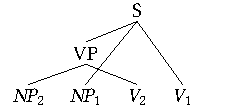
\includegraphics{graphics/abb63.pdf}
\caption{\label{fig-ttmctag-kohaerenz-2}Beispiel einer direkten Repräsentation einer diskontinuierlichen Valenzrealisierung}
\end{figure}

Einer kanonischen CFG am nächsten kommen wohl CFG-Derivate, die zusätzliche, weniger strikte Linearisierungsoperatoren für die rechte Regelseite einführen. Zu nennen sind hier etwa DPSG \citep{Bunt:etal:87}, LSL \citep{Suhre:99}, oder poms-CFG \citep{Nederhof:etal:03}. Die zwei LSL-Regeln (Linear Spezification Language) in \ref{ex-koharenz-strategien-1} beispielsweise erfassen die diskontinuierliche Struktur in Abbildung \ref{fig-ttmctag-kohaerenz-2}, wobei nicht-unmittelbare Präzedens durch den Operator < anzeigt wird:\footnote{\cite{Suhre:99} verwendet zunächst eine ID/LP-artige Notation. Da die LP-Spezifikationen jedoch immer regelbezogen sind, lassen sie sich mit den ID"=Spezifikationen zusammenfassen.}  

\ex. \label{ex-koharenz-strategien-1}
S $\to$ VP {\it NP$_1$} < {\it V$_1$} \\
VP $\to$ {\it NP$_2$} < {\it V$_2$}

Man beachte, dass die Position des VP-Nichtterminals in der ersten Regel vollkommen unterspezifiziert ist und deshalb der dazugehörige Yield (also {\it NP$_2$} und {\it V$_2$} der zweiten Regel) diskontinuierlich sein kann.
	
Einen anderen Weg gehen CFG-Derivate, die Yield-Funktionen verwenden, z.\,B.\ LCFRS\is{Linear Context-Free Rewriting Systems (LCFRS)} \citep{Vijay-Shanker:etal:87,Weir:88}, MCFG \citep{Seki:etal:91}, LMG \citep{Groenink:95} und RCG \citep{Boullier:00}.\footnote{Siehe \citet[Abschnitt~2.2]{Kallmeyer:10} für eine Übersicht über deren formale Eigenschaften.} Bei einer RCG (Range Concatenation Grammar) werden die Yield-Funktionen direkt in die Regeln geschrieben. Die RCG-Regeln unterscheiden sich oberflächlich von CFG-Regeln nur insofern, als statt der Nichtterminale Prädikate über Terminalketten verwendet werden. Für die Erfassung der diskontinuierlichen Struktur in Abbildung \ref{fig-ttmctag-kohaerenz-2} genügen die beiden RCG-Regeln in \ref{ex-koharenz-strategien-2}:  

\ex. \label{ex-koharenz-strategien-2}
S(X {\it NP$_1$} Y {\it V$_1$}) $\to$ VP(X,Y) \\
VP({\it NP$_2$},{\it V$_2$}) $\to$ $\epsilon$
 
X und Y sind sogenannte Range-Variablen, die einen zusammenhängende Bereich in der Terminalkette denotieren.\footnote{Genaugenommen sind Range-Variablen Variablen über Paaren natürlicher Zahlen, die den Start- und Endpunkt eines Stringbereichs festlegen.} Das S-Prädikat in der ersten Regel ist einstellig, erlaubt es aber, das Argument, d.\,h.\ eine Terminalkette, mittels Range-Variablen und Terminale zu unterteilen und die Range-Variablen in den Prädikaten auf der rechten Regelseite wiederzuverwenden. Die Diskontinuität kommt dann im VP-Prädikat zum Vorschein, wo die Argumente nicht-adjazente Bereiche der Terminalkette sind.

Schlie\ss lich besteht die Möglichkeit, den ID/LP-Ansatz aus \cite{Gazdar:Pullum:81} und \cite{Shieber:84} weiterzuentwickeln. ID/LP stellt im Grunde eine Methode dar, mittels unterschiedlicher Regeltypen, d.\,h.\ Regeln der unmittelbaren Dominanz (ID) und Regeln der linearen Präzedens (LP), die Menge der Regeln einer CFG zu faktorisieren. Da ID/LP und CFG schwach äquivalent sind, ist auch ID/LP grundsätzlich nicht in der Lage, diskontinuierliche Strukturen zu erzeugen. Ursache dafür ist letztlich die implizite Zusatzannahme, dass von einem Knoten dominierte Knoten kontinuierlich linearisiert sind. Gibt man diese Zusatzannahme auf, kann Diskontinuität sehr wohl direkt repräsentiert werden.\footnote{Ein alternatives Vorgehen zeigt \cite{Pullum:82}: Mittels einer Metaregel ("`liberation"') wird ausgehend von einer Dominanzregel S $\to$ VP {\it NP$_1$} {\it V$_1$} eine Dominanzregeln S $\to$ {\it NP$_2$} {\it V$_2$} {\it NP$_1$} {\it V$_1$} hinzugenommen, falls es eine Dominanzregel VP $\to$ {\it NP$_2$} {\it V$_2$} gibt. {\it NP$_2$} und {\it V$_2$} werden also quasi aus VP "`befreit"'. Siehe dazu auch \citet[81f]{Kathol:95} und \citet[32f]{Kathol:00}.} Die ID/LP-Spezifikationen in \ref{ex-koharenz-strategien-3} lizenzieren dann unter anderem die Struktur in Abbildung \ref{fig-ttmctag-kohaerenz-2}: 

\ex. \label{ex-koharenz-strategien-3} 
\a. S $\to$ VP {\it NP$_1$} {\it V$_1$} \\
VP $\to$ {\it NP$_2$} {\it V$_2$}
\b. \label{ex-koharenz-strategien-3-b} {\it NP} < {\it V}

Man beachte, dass die LP-Spezifikation in \ref{ex-koharenz-strategien-3-b} global gilt, d.\,h.\ für beide ID"=Spezifikationen (weshalb die Indizierung hier fehlt). Darin liegt der wesentliche Unterschied zu LSL, wo nur lokale LP-Spezifikationen möglich sind. Einen solcherart unrestringierten ID/LP-Ansatz, der kreuzende Kanten zulässt, verfolgen  beispielsweise der Direct-Liberation-Ansatz von \cite{Zwicky:86}, Mobile Grammars \citep{Blevins:90} und Generalized ID/LP \citep{Daniels:05}. Hinzu kommt jeweils eine Domänenspezifikation, um Diskontinuität effektiv zu regulieren.

Auf den ersten Blick gehört auch der Linearisierungsansatz für HPSG\is{Head-driven Phrase Structure Grammar (HPSG)}, den Mike Reape \citep{Reape:92,Reape:94,Reape:96} ausgearbeitet hat, in diese Gruppe der ID/LP-Ansätze: Die lineare Präzedens der Terminale ergibt sich nicht aus der Dominanzstruktur, wie bei HPSG sonst der Fall. Stattdessen wird sie durch das Zusammenspiel von LP-Spezifikationen und Domänenspezifikationen lizenziert. Doch auf den zweiten Blick erkennt man einen wesentlichen Unterschied zu Mobile Grammars und Generalized ID/LP: Die Dominanzstrukturen bei Reape sind ungeordnete Bäume, die mit der Terminalkette nur indirekt verbunden sind. Dagegen generieren obige ID/LP-Ansätze linear geordnete Phrasenstrukturen mit den Terminalen als Blätter. 

Ein Beispiel soll dies verdeutlichen. In Abbildung \ref{fig-kohaerenz-strategien-2} sieht man eine stark verkürzte HPSG-Repräsentation für den indizierten String {\it NP$_2$ NP$_1$ V$_2$ V$_1$}, in der Reapes Merkmal {\sc dom} für die Linearisierung der Terminale zuständig ist. Der {\sc dom}-Wert ist eigentlich eine Liste von {\it sign}-Objekten, aber ich beschränke mich hier auf die Angabe derer {\sc phon}-Werte. Die {\sc dom}-Liste eines Mutterknotens wird aus den {\sc dom}-Listen der Tochterknoten mit Hilfe des $\ocircle$-Operators ("`shuffle"', "`sequence-union"') zusammengesetzt, wobei LP-Beschränkungen beachtet werden müssen.\footnote{Bei Reape beziehen sich die LP-Beschränkungen auf die syntaktische Kategorie der {\sc dom}-Listenelemente. \cite{Kathol:95,Kathol:00} benutzt hier stattdessen Marker für topologische Felder. Siehe auch \cite{Mueller:96,Mueller:99,Mueller:02,Mueller:04}, der den Reapeschen Linerarisierungsansatz in seinem Babel-System (\url{http://hpsg.fu-berlin.de/~stefan/Babel/}) verwendet. Man beachte, dass Kathol und Müller einen hybriden Linearungsansatz implementieren, mit  Valenzvereinigung im Verbalkomlex und Extraktion ins Vorfeld. Ein Linearisierungsansatz anderer Art wird in \cite{Richter:Sailer:95} und \cite{Richter:97} vorgeschlagen. Die "`Permutationsdomäne"'  entspricht dort nicht einer {\sc dom}-Liste in der Merkmalsstruktur einer Phrase, sondern einer {\sc phon}-Liste, die durch die zweistellige Relation {\tt perm-domain} mit einer Phrase in Verbindung gebracht wird. Richter und Sailer zeigen au\ss erdem, dass der Linearisierungsansatz durchaus mit Valenzvereinigungsansätze wie \cite{Hinrichs:Nakazawa:94} kombinierbar ist. Es darf jedoch bezweifelt werden, dass ein direkter Modellierungsansatz im Rahmen der HPSG\is{Head-driven Phrase Structure Grammar (HPSG)} ohne Linearisierungsmodul auskommt.} Die {\sc dom}-Liste des S-Knotens entspricht dann der Terminalkette im üblichen Sinne, wovon jedoch die Dominanzstruktur unbeeinflusst ist. Gekreuzte Kanten\is{kreuzende Kante} ergeben sich hier nur bei einer Abbildung der Blätter auf die dazugehörigen Elemente der {\sc dom}-Liste im S-Knoten, wie in Abbildung \ref{fig-kohaerenz-strategien-2} zu sehen ist.   

\begin{figure}[t]
\centering
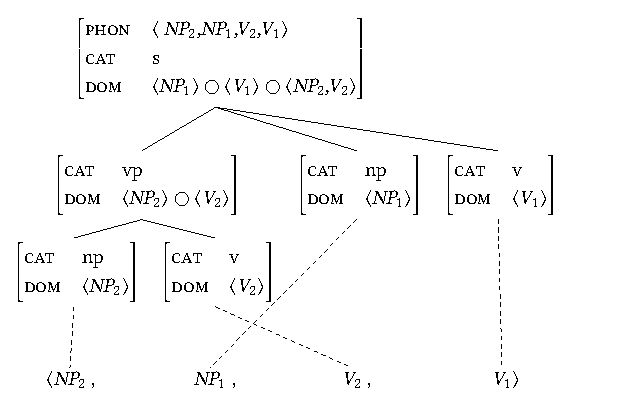
\includegraphics{graphics/abb64.pdf}
\caption{\label{fig-kohaerenz-strategien-2}Direkte HPSG-Repräsentation einer diskontinuierlichen Valenzrealisierung mit den Linearisierungsdomänen aus \cite{Reape:92,Reape:94,Reape:96}}
\end{figure}
 
Bei dieser doppelten repräsentationellen Trennung von Dominanz und Linearisierung beruft sich die HPSG-\is{Head-driven Phrase Structure Grammar (HPSG)} und CG-Literatur\is{Kategorialgrammatik}\footnote{Im CG-Bereich ist vor allem die Abstract Categorial Grammar (ACG) hervorzuheben, die \cite{deGroote:01} und \cite{Muskens:01} einführen.} auf die Unterscheidung zwischen \textsc{Tektogrammatik}\is{Tektogrammatik} und \textsc{Phänogrammatik}\is{Phänogrammatik} in \citet[65f]{Curry:63}:\footnote{Vgl.\ auch \citet[12ff]{Dowty:96} und \citet[35ff]{Kathol:00}.} Die Tektogrammatik beschreibt die Dominanzstruktur (bzw.\ bei Curry die Funktor"=Argument"=Struktur) eines Satzes, die Phänogrammatik dagegen dessen Linearisierung. Beide Grammatikdimensionen gelten als parallel in dem Sinne, dass keine generative Ordnung zwischen ihnen besteht -- anders als etwa bei der Transformationsgrammatik, wo die \isi{Oberflächenstruktur} aus der \isi{Tiefenstruktur} abgeleitet wird. 


Eine vergleichbare Trennung findet sich jedoch schon bei \cite{Tesniere:59}, wo strukturale Ordnung ("`ordre structural"'), d.\,h.\ die ungeordnete Dependenzstruktur\is{Dependenzgraph}, und linearer Ordnung ("`ordre lin\'eaire"') gegenüberstellt werden.\footnote{Deutsche Terminologie nach \citet[33]{Agel:00}.} Es ist deshalb nicht verwunderlich, dass man eine Trennung von Dominanz und Linearisierung auch in Arbeiten im Rahmen der \isi{Dependenzgrammatik} antrifft. So ist es bei der Extensible Dependency Grammar (XDG, \citealt{Duchier:Debusmann:01, Debusmann:etal:04}) möglich, "`Dimensionen"' der linguistischen Beschreibung mit je unterschiedlichen Gesetzmä\ss igkeiten zu definieren, etwa einen syntaktischen Dependenzgraphen ("`ID tree"') und einen topologischen Dependenzgraphen ("`LP tree"'). Die topologische Repräsentation bildet hier allerdings nicht nur die lineare Ordnung ab (allein durch die Tatsache, dass der topologische Dependenzgraph geordnet ist), sondern stipuliert auch eine partielle hierarchische Ordnung der Wörter anhand der Zugehörigkeit zu einem topologischen Feld. Beispielsweise dominieren Verben in der linken Satzklammer die Bestandteile des Vorfelds, des Mittelfelds und der rechten Satzklammer. Diese hierarchische Ordnung der topologischen Felder ist ein Resultat der Modellierung mittels Dependenzgraphen und eigentlich unüblich. \cite{Gerdes:Kahane:01} gehen in ihrem mehrdimensionalen Ansatz in dieser Hinsicht anders vor, indem die Topologie stattdessen durch ein lineares Felderschema repräsentiert wird und hierarchische Aspekte nur durch Einbettungsverhältnisse einflie\ss en. 


\subsection{Und TAG?}

TAG kann durch die erweiterte Lokalitätsdomäne kreuzende Abhängigkeiten\is{kreuzende Abhängigkeit} und eingeschränkt auch \isi{Scrambling} in kohärenten Konstruktionen\is{kohärente Konstruktion} direkt erzeugen (siehe Abschnitt~\ref{sec-tag-grenzen-scram}). Dazu zählt auch die indizierte Terminalkette (bzw.\ das String-Schema) {\it NP$_2$ NP$_1$ V$_2$ V$_1$}, wobei sich allerdings im dazugehörigen abgeleiteten Baum keine kreuzenden Kanten\is{kreuzende Kante} befinden können. Sie werden nur sichtbar, wenn eine bestimmte Variante des Ableitungsbaums auf die Terminalkette abgebildet wird. Dies geschieht etwa in Abbildung \ref{fig-kohaerenz-strategien-3}, wo das Dominanzverhältnis zwischen $\gamma_1$ und $\gamma_2$ im Ableitungsbaum im Vergleich zur üblichen Notation invertiert ist. Dank dieser generativen Ausdrucksstärke implementieren die meisten TAG-Analysen kohärenter Konstruktionen einen direkten Valenzrealisierungsansatz. Dazu mehr im nächsten Abschnitt.   

\begin{figure}
\centering
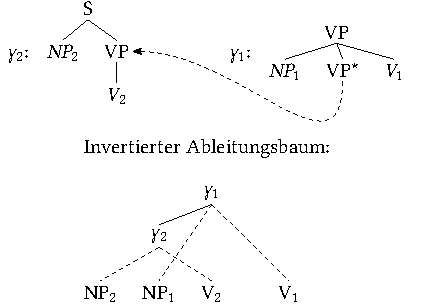
\includegraphics[angle=90]{graphics/abb65.pdf}
\caption{\label{fig-kohaerenz-strategien-3}Direkte Ableitung einer diskontinuierlichen Valenzrealisierung mit TAG}
\end{figure}

Neben einer direkten Realisierung diskontinuierlicher Valenzrahmen ist es aber auch möglich, einen Bewegungsansatz\is{Bewegung} mit Baummengen zu implementieren, die das bewegte Element und seine Spur bündeln. Kallmeyer motiviert mit einer solchen Modellierungsmöglichkeit eine MCTAG-Variante, SN-MCTAG, auf die ich in Abschnitt \ref{sec-snmctag} eingehen werde. 

Ein Valenzvereinigungsansatz\is{Valenzvereinigung} ist dagegen nicht durchführbar. Das scheitert an der fundamentalen Unfähigkeit des TAG-Formalismus, nichtterminale Blätter eines Elementarbaums während der Ableitung zu tilgen oder neue hinzuzufügen. Dadurch fehlt einer Abstraktion der Valenzrepräsentation die formale Voraussetzung, wie sie etwa in der HPSG\is{Head-driven Phrase Structure Grammar (HPSG)} mittels Listenmanipulation vorhanden ist. Auch bei \citet[171]{Rambow:94} liegt keine Valenzvereinigung im eigentlichen Sinne vor: Wenn dort die Valenzrahmen kohärent konstruierender Verben in einer Baummenge dargestellt werden, spiegelt diese Darstellung  einen Zustand in der Ableitung wieder. Die Baummengen haben jedoch keinen lexikalischen Status, was u.\,a.\ bedeutet, dass das regierende Verb keinen direkten Zugriff auf die Argumentbäume des regierten Verbs hat. Die Kasusmarkierung bei Anhebungskonstruktionen wie dem Fernpassiv\is{Passiv!Fern-} muss also weiterhin indirekt über \isi{Merkmalsperkolation} im abgeleiteten Baum erfolgen (siehe S.~\pageref{sec-ttmctag-fern}f). Au\ss erdem, so lässt sich vermuten, müsste es für einen echten Vertreter des Valenzvereinigungsansatzes möglich sein, auf eine explizite Spezifizierung der Lokalitätsdomäne mittels Integrity Constraints\is{Integrity Constraint} zu verzichten (siehe Abschnitt~\ref{sec-tag-varianten-vtag}).




\section{TAG-Varianten für das Deutsche} \label{sec-tag-varianten}

Die ungenügende derivationelle Mächtigkeit des TAG-Formalismus bei der Modellierung von Scrambling-Phänomenen wurde in Abschnitt~\ref{sec-tag-grenzen} deutlich.\footnote{Eine große implementierte Grammatik des Deutschen, die trotz allem auf TAG basiert, ist DTAG \citep{Gerdes:02,Gerdes:02b}. Gerdes rechtfertigt seine Wahl und die damit einhergehenden Abdeckungslücken damit, dass die Grammatik vornehmlich zur Textgenerierung entwickelt wurde und außerdem zu jener Zeit die Software für mächtigere MCTAG-Varianten nicht zur Verfügung stand. Letzteres hat sich aber mittlerweile geändert \citep{Parmentier:etal:07,Kallmeyer:etal:08}. Die große Menge an TAG-Baumschablonen, die den vielen Stellungsmöglichkeiten der Verben und ihrer Argumente geschuldet ist, generiert Gerdes mit einer sogenannten Metagrammatik. Man beachte, dass die Grammatik bei MCTAG-Varianten erheblich kleiner ausfallen kann.} Um dem abzuhelfen, kam es in den letzten zwei Jahrzehnten zur Ausarbeitung mehrerer TAG- und MCTAG-Erweiterungen. Ganz am Anfang standen ID/LP"=Ansätze, die durch die Unterspezifizierung der linearen Präzedens der Blätter eines Elementarbaums die Generierung kreuzender Kanten zulassen. Dazu zählen LD/LP-TAG (\citealt{Joshi:87b, Joshi:etal:90}) und FO-TAG (\citealt{Becker:Joshi:Rambow:91, Becker:94}).\footnote{Siehe \citet[43ff]{Rambow:94} für eine kritische Auseinandersetzung mit FO-TAG.} Für den Zweck der linguistischen Modellierung haben sich schlie\ss lich Ansätze durchgesetzt, die im Wesentlichen eine Unterspezifizierung der Dominanzverhältnisse gemeinsam haben. Zwei Richtungen lassen sich hier unterscheiden: Zum einen gibt es Erweiterungen wie V-TAG\is{Vector-MCTAG (V-TAG)} \citep{Rambow:94} und TUG\is{Tree Unification Grammar (TUG)} \citep{Gerdes:04}, die von einer NL-MCTAG ausgehen und diese modifizieren; zum anderen gibt es Versuche, reguläre TAG oder TL-MCTAG möglichst minimal zu erweitern, so dass die benötigte generative und derivationelle Mächtigkeit erzielt wird. Hierunter fallen DTG\is{D-Tree Grammar (DTG)} \citep{Rambow:etal:95}, SegTAG\is{Segmented TAG (SegTAG)} \citep{Kulick:00} und SN-MCTAG\is{TL-MCTAG with Shared Nodes (SN-MCTAG)} \citep{Kallmeyer:05}. Mein eigener Vorschlag, \isi{TT-MCTAG}, kann wohl eher der letzteren  Richtung zugeordnet werden, zeigt aber auch Ähnlichkeiten zu V-TAG. Eine ausführliche Darstellung von TT-MCTAG folgt in Kapitel \ref{sec-ttmctag}. 

\subsection{V-TAG} \label{sec-tag-varianten-vtag}\is{Vector-MCTAG (V-TAG)|(}

Wie bereits in Abschnitt~\ref{sec-tag-grenzen-scram} angesprochen, schlägt \cite{Rambow:94} für die Modellierung von Scrambling in kohärenten Konstruktionen eine Variante der nicht-lokalen MCTAG (NL-MCTAG)\is{Multi-Component TAG (MCTAG)!nichtlokale (NL-MCTAG)} vor, die er als Vector-MCTAG, oder kurz V-TAG bezeichnet. Der wesentliche Unterschied zwischen NL-MCTAG und V-TAG ist der, dass V-TAG, anders als NL-MCTAG, eine nicht-simultane Verknüpfung der Elemente einer Baummenge erlaubt. Diese Modifikation wirkt sich positiv auf die computationelle Komplexität des Formalismus aus:\footnote{Man möchte sagen, überraschenderweise, da V-TAG weniger beschränkt ist als NL-MCTAG\is{Multi-Component TAG (MCTAG)!nichtlokale (NL-MCTAG)}. Die Beschränkung durch die \isi{Simultanitätsbedingung}, d.\,h.\ deren Überprüfung, scheint jedoch sehr aufwändig zu sein und nicht effektiv den Suchraum zu verkleinern.} Rambow kann zeigen, dass das Parsen mit jeder (fixierten) V-TAG polynomielle Zeitkomplexität hat \citep[120ff]{Rambow:94}, während das für NL-MCTAG\is{Multi-Component TAG (MCTAG)!nichtlokale (NL-MCTAG)} mit \isi{Simultanitätsbedingung} nicht gilt \citep{Rambow:Satta:92,Champollion:11a}. 

Durch das Fehlen der Simultanitätsbedingung ist au\ss erdem die derivationelle Mächtigkeit\is{derivationelle Mächtigkeit} signifikant erhöht. Deutlich wird das beispielsweise bei der Ableitung von Satz \ref{ex-vtag-1} (bzw.\ \ref{ex-schema2} auf S.~\pageref{ex-schema2}) mittels der Baummengen in Abbildung~\ref{fig-vtag-1}:

\exg. {Dieses Buch} hat {den Kindern} niemand {zu geben} versucht.  \\
$\mathit{NP}_2$ $V1_1$ $\mathit{NP}_2$ $\mathit{NP}_1$ $V_2$ $V_1$ \\
\citep[42]{Rambow:94} \label{ex-vtag-1}

\begin{figure}[t]
\centering
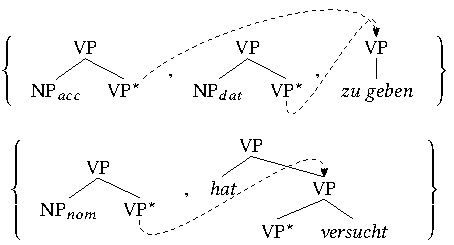
\includegraphics{graphics/abb66.pdf}
\caption{V-TAG-Baummengen für die Derivation des Satzes in \ref{ex-vtag-1}\label{fig-vtag-1}}
\end{figure}
Dabei muss nämlich der Hilfsbaum mit NP$_{nom}$-Blatt direkt an den Baum von {\it hat versucht} adjungieren, was klar der \isi{Simultanitätsbedingung} widerspricht.

Ebenfalls positiv wirkt sich dieser Zugewinn an derivationeller Mächtigkeit\is{derivationelle Mächtigkeit} beim Entwurf der Baummengen für die indizierten Sprache $\mathsf{SCR}^{ind}$ aus. Hierfür genügen nämlich die beiden Baummengen in Abbildung~\ref{fig-vtag-2}, da Elemente aus einer Baummenge untereinander verknüpft werden können.  
\begin{figure}[t]
\centering
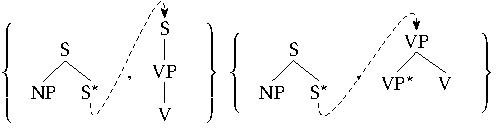
\includegraphics{graphics/abb67.pdf}
\caption{V-TAG-Baummengen für die indizierte Sprache $\mathsf{SCR}^{ind}$\label{fig-vtag-2}}
\end{figure}
Die gestrichelten Pfeile stehen hier für Dominanzlinks\is{Dominanzlink}, die im abgeleiteten Baum überprüft werden. Zusätzlich verfügt V-TAG über die Möglichkeit, die Knoten mit {\it Integrity Constraints}\is{Integrity Constraint} (d.\,h.\ mit $\bigtriangleup$) zu versehen, über die kein Dominanzlink verlaufen darf. Dominanzlinks und Integrity Constraints sind ein wichtiges Mittel der Einschränkung der Nicht-Lokalität. Sie spielen aber auch eine Rolle bei der Anpassung der valenzbezogenen Wohlgeformtheitsbedinungen\is{Wohlgeformtheitsprinzip} für Baummengen. Dazu kommen wir jetzt. 

Aus valenztheoretischer Perspektive -- die Baummengen in Abbildung~\ref{fig-vtag-1} und Abbildung~\ref{fig-vtag-2} haben es exemplarisch gezeigt -- gewinnt man den Eindruck, dass es ohne \isi{Simultanitätsbedingung} leichter fällt, Valenzrahmen in Baummengen aufzutrennen. Dagegen eignen sich simultane MCTAG wie die Weir'sche Varianten, aber auch SN-MCTAG\is{TL-MCTAG with Shared Nodes (SN-MCTAG)} (siehe Abschnitt~\ref{sec-snmctag}), besser für Bewegungsanalysen\is{Bewegung}, bei denen der Valenzrahmen im Normalfall durch einzelne Elementarbäume repräsentiert wird. Wenn aber die Elementarbaummenge und nicht mehr der Elementarbaum den Bereich definiert, in dem Valenzbeziehungen zum Ausdruck kommen, dann müssen die Wohlgeformtheitsprinzipien\is{Wohlgeformtheitsprinzip} mit Valenzbezug dem angepasst werden. Rambow bezieht sich hier allerdings auf die Wohlgeformtheitsprinzipien in \cite{Frank:92}, worin noch kein $\theta$-Kriterium \`a la \ref{ex-cetm} zu finden ist,\footnote{Stattdessen gibt es ein "`Projection Principle"' \citep[56]{Frank:92}.} definiert ein $\theta$-Kriterium für V-TAG\is{Wohlgeformtheitsprinzip!theta-Kriterium für V-TAG@$\theta$-Kriterium für V-TAG}\footnote{"`The $\theta$-Criterion (V-TAG version): frontier nonterminal nodes in a lexical set are assigned $\theta$-roles by its lexcial head. Furthermore, all $\theta$-roles of the head are discharged in this manner."' \citep[148]{Rambow:94}} und vermengt es mit Franks CETM. Das Ergebnis sieht folgenderma\ss en aus:\is{Wohlgeformtheitsprinzip!CETM für V-TAG}
    
\ex. The {\bf Condition on Elementary Tree Minimality} (V-TAG version, final): every lexical set contains exactly one lexical head. There is a bijection between $\theta$-roles the head assigns and the frontier nonterminal nodes of the set. \citep[149]{Rambow:94} \label{ex-vtag-cetm}

Es fällt zunächst auf, dass der explizite Bezug zur erweiterten Projektion\is{erweiterte Projektion}, der im ursprünglichen CETM in \cite{Frank:92,Frank:02} zentral ist, in dieser Version des CETM fehlt. Er verbirgt sich allerdings hinter der ersten Klausel "`every lexical set contains exactly one lexical head"'. Der lexikalische Kopf bestimmt nämlich durch Merkmalsprojektion (geregelt durch das "`Head Feature Principle"' \citealt[141f]{Rambow:94}) die Knoten-Label der Projektion. Hinzu kommt noch ein weiteres Prinzip, das die Struktur der Elementarbaummenge einschränkt ("`lexical set structure principle"', \citealt[149]{Rambow:94}). Demnach soll z.\,B.\ jedes $\theta$-markierte, nicht-terminale Blatt einen eigenen Elementarbaum bilden, indem dieses mit einer Projektionskante kombiniert wird (wie in Abbildung~\ref{fig-vtag-1}). Auf die Details dieser strukturellen Regelungen möchte ich aber hier nicht weiter eingehen. Wichtig für uns ist die zweite Klausel aus Rambows CETM, die im Grunde eine angepasste Form des $\theta$-Kriteriums aus \ref{ex-theta-criterion} darstellt. Klärungsbedürftig ist allerdings die Bedeutung des Ausdrucks "`frontier nonterminal nodes of the set"', denn die Baummengen in Abbildung~\ref{fig-vtag-1} und \ref{fig-vtag-2} besitzen mehr nicht-terminale Blätter als $\theta$-Markierungen\is{theta-Markierung@$\theta$-Markierung}, was zwingend aus der Auf"|teilung des $\theta$-Rasters auf unterschiedliche Elementarbäume innerhalb einer Baummenge folgt. Tatsächlich sind nur diejenigen nicht-terminalen Blätter $\theta$-markiert, die nicht Ausgangspunkt eines Dominanzlinks\is{Dominanzlink} sind.\footnote{"`the frontier nodes are the nonterminals [\ldots] in which no dominance links originate"' \citep[148, Fußnote~14]{Rambow:94}.} Das hei\ss t im Umkehrschluss, dass alle nicht-terminalen Knoten, die nicht $\theta$-markiert sind, einen ausgehenden Dominanzlink haben müssen.  

Mit V-TAG steht ein mächtiges Werkzeug für die Modellierung von kohärenten Konstruktionen zur Verfügung, was angesichts der Nicht-Lokalität des Formalismus nicht verwundert. Doch obwohl diese nicht-simultane Nicht-Lokalität im Rahmen des computationell Erwünschten bleibt, sind in der Literatur kritische Stimmen laut geworden, die an bestimmten Begleiterscheinungen Ansto\ss \ nehmen (z.\,B.\ \citealt[60]{Kulick:00}; \citealt[239]{Frank:02}; \citealt[191]{Kallmeyer:05}). Demnach sei der Grundgedanke von TAG, Lokalität allein mittels Elementarstrukturen und deren Verknüpfung herzustellen, durch die zusätzliche Annahme von Dominanzlinks\is{Dominanzlink} und Integrity Constraints\is{Integrity Constraint} geschwächt, wenn nicht gar ersetzt. Damit folgt nämlich die Lokalität syntaktischer Beziehungen nicht mehr aus unabhängig motivierten Prinzipien, sondern muss explizit stipuliert werden.
\is{Vector-MCTAG (V-TAG)|)}  


\subsection{DTG} \label{sec-dtg}\is{D-Tree Grammar (DTG)|(}

D-Tree Grammar (DTG, \citealt{Rambow:etal:95}) steht für den Versuch, zwei Unzulänglichkeiten des TAG-Kernformalismus zu überwinden: (i) die eingeschränkte \isi{derivationelle Mächtigkeit} bei Diskontinuitätsphänomenen und (ii) die Diskrepanz zwischen \isi{Ableitungsbaum} und \isi{Dependenzgraph} (siehe S.~\pageref{sec-ableitungsbaum}). In diesem Abschnitt werde ich nur auf den ersten Punkt eingehen.\footnote{Eine ausführlichere Formalisierung der DTG als Baumbeschreibungensgrammatik (in Anlehnung an \citealt{Vijay-Shanker:92}) liefern \cite{Rambow:etal:01} nach, wobei sie im Vergleich zu \cite{Rambow:etal:95} umfassende terminologische Änderungen vornehmen. Die DTG hei\ss t dort D-Tree Substitution Grammar (DSG), die Verknüpfungsoperation bei Komplementation wird "`generalized substitution"' genannt, die durch "`path constraints"' kontrolliert wird. Ich bleibe hier der Terminologie aus \cite{Rambow:etal:95} treu. Ein schwerwiegender Unterschied zwischen DTG und DSG könnte darin bestehen, dass DTG nur baumförmige D-Trees zulässt, DSG dagegen auch nicht-baumförmige D-Trees. Eine Alternative zur DTG bzw.\ DSG schlägt \cite{Kallmeyer:01} mit der Local Tree Descritption Grammar (TDG) vor, vornehmlich unter dem Gesichtspunkt der Diskontinuitätsmodellierung. Da die konzeptuellen Unterschiede zwischen DTG und TDG marginal sind (siehe \citealt[118]{Rambow:etal:01}), möchte ich auf die TDG an dieser Stelle nicht weiter eingehen.}

Eine DTG besteht nicht aus Elementarbäumen im herkömmlichen Sinn, sondern aus sogenannten \textsc{D-Trees}. D-Trees besitzen nicht nur Kanten für unmittelbare Dominanz, sogenannte i-Kanten ("`i-edges"'), sondern auch d-Kanten ("`d-edges"'), d.\,h.\ Kanten, die ein unterspezifiziertes Dominanzverhältnis ausdrücken. Mittels dieser d-Kanten können die Elementarbäume aufgebrochen werden und Fragmente anderer D-Trees intervenieren. Für die Modellierung des Beispielsatzes in \ref{ex-vtag-1}, hier nochmal wiederholt als \ref{ex-dtg-1}, können beispielsweise die D-Trees in Abbildung \ref{fig-dtg-1} herangezogen werden: 

\ex. {Dieses Buch} hat {den Kindern} niemand {zu geben} versucht. \label{ex-dtg-1}

\begin{figure}[t]
\centering
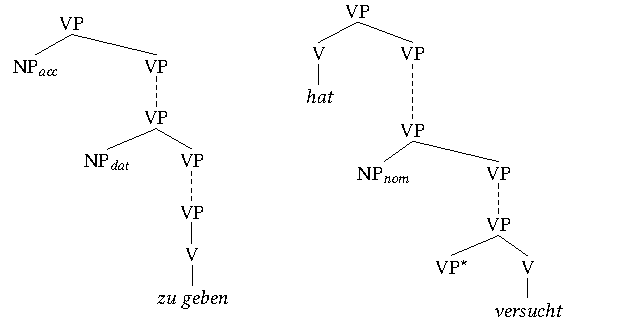
\includegraphics{graphics/abb68.pdf}
\caption{\label{fig-dtg-1}D-Trees für die Derivation von \ref{ex-dtg-1}}
\end{figure}
Die d-Kanten, die hier gestrichelt dargestellt werden, verbinden sogenannte D-Tree-Kompo\-nenten, d.\,h.\ Teilbäume mit i-Kanten. Um D-Trees zu verknüpfen, entwerfen \cite{Rambow:etal:95} eine spezielle Verknüpfungsoperation: die \textsc{Subsertion}.\footnote{In \cite{Rambow:etal:01} wird die Subsertion in "`generalized substitution"' umbenannt.} Dabei handelt es sich um eine zweiteilige Operation aus klassischer Substitution und "`insertion"', d.\,h.\ dem Einfügen von D-Tree-Komponenten in d-Kanten. Der Unterschied ist schematisch in Abbildung \ref{fig-dtg-3} veranschaulicht. Während die $\alpha_2$-Komponente ein Blatt der $\beta_2$-Komponente substituiert, wird die dominierende $\alpha_1$-Komponente in die d-Kante des $\beta$-Baums eingesetzt. 
\begin{figure}
\centering
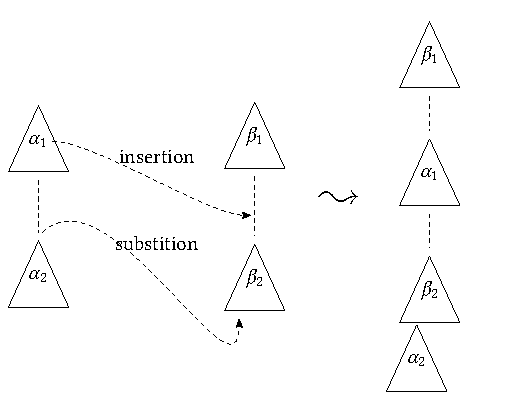
\includegraphics{graphics/abb69.pdf}
\caption{\label{fig-dtg-3}Schema der Subsertion}
\end{figure}
Neben der Subsertion kann bei der D-Tree-Verknüpfung in Fällen der Modifikation auf die Schwester-Adjunktion ("`sister-adjunction"') aus \cite{Schabes:Shieber:94} zurückgegriffen werden. Wendet man die Subsertion auf die D-Trees in Abbildung \ref{fig-dtg-1} an, dann ist die Ableitung der Phrasenstruktur in Abbildung \ref{fig-dtg-2} möglich, und damit die Ableitung des für TAG problematischen Satzes in \ref{ex-dtg-1}.
\begin{figure}[t]
\centering
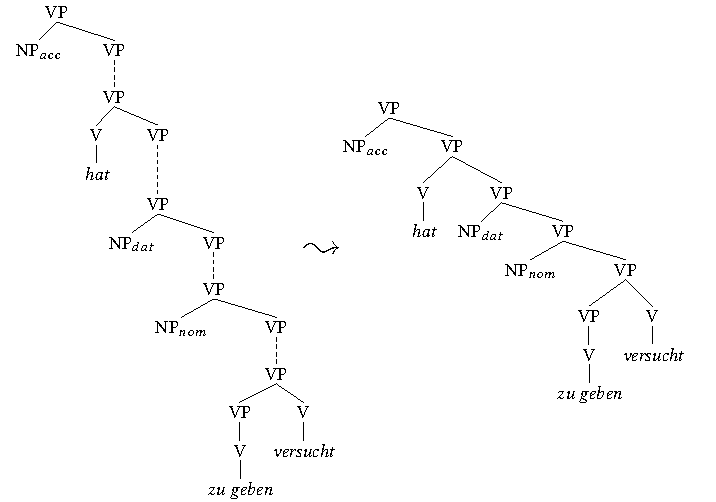
\includegraphics{graphics/abb610.pdf}
\caption{\label{fig-dtg-2}Abgeleiteter Baum nach Subsertion der D-Trees aus Abbildung~\ref{fig-dtg-1}}
\end{figure}

Die Subsertion von D-Trees ist so ausdrucksstark, dass damit sogar die \isi{MIX-Sprache} generiert werden kann \citep[Abb.~13]{Rambow:etal:01}, was auch die Möglichkeit zur Generierung von $\mathsf{SCR}^{ind}$\is{indizierte Scramblingsprache ($\mathsf{SCR}^{ind}$)} einschlie\ss t. Um diesen potenten Mechanismus zu kontrollieren, stellen \cite{Rambow:etal:95} zwei Beschränkungswege zur Verfügung: Zum einen soll nur genau ein Wurzelknoten einer D-Tree-Komponente substituierbar ("`substitutable"') sein, um baumförmige Ableitungsgraphen zu erhalten und das Zustandekommen mehrerer Valenzbeziehungen zwischen zwei Elementen zu verhindern; zum anderen kann man "`subsertion-insertion constraints"' (SIC) auf den d-Kanten definieren. Eine SIC für eine d-Kante $\langle v_1,v_2 \rangle$ eines D-Trees $\gamma$ spezifiziert, welche Knoten anderer D-Trees nicht auf dem Dominanzpfad zwischen $v_1$ und $v_2$ liegen dürfen.\footnote{\cite{Rambow:etal:01} nennen die SICs deswegen auch viel treffender "`path constraints"'.} Nur dadurch ist die Lokalität der D-Tree-Komponenten im abgeleiteten Baum expressis verbis eingrenzbar.

DTG erinnert stark an V-TAG. Die Ähnlichkeit zwischen den D-Trees in Abbildung \ref{fig-dtg-1} und den V-TAG-Baummengen in Abbildung \ref{fig-vtag-1} für die Modellierung der kohärenten Konstruktion in \ref{ex-dtg-1} ist frappierend. Beide Formalismen verwenden in unterschiedlicher aber entsprechender Weise unterspezifizierte Dominanzrelation, deren Einschränkung spezifisch für jede einzelne Elementarstruktur durch einen zusätzlichen Mechanismus (SIC hier, Integrity Constraints\is{Integrity Constraint} dort) zu erfolgen hat. In dieser Hinsicht greift bei DTG also derselbe Kritikpunkt, der oben bei der Darstellung von V-TAG genannt wurde: Die Lokalität syntaktischer Beziehungen folgt nicht mehr aus der Form der Elementarstrukturen und den Verknüpfungsoperationen, sondern muss explizit stipuliert werden.  
\is{D-Tree Grammar (DTG)|)}


\subsection{SegTAG}\is{Segmented TAG (SegTAG)|(}

Segmented Tree Adjoining Grammar (SegTAG) ist eine TAG-Erweiterung, die \cite{Kulick:00} in erster Linie zur Analyse des Clitic Climbings in romanischen Sprachen und zur Analyse des Scramblings in kohärenten Konstruktionen des Deutschen einsetzt. Motiviert wird SegTAG jedoch auch mit bestimmten Phänomenen bei Subjekt-Anhebung im Englischen, die sowohl für TAG als auch für TL-MCTAG (in einem CP-IP-Strukturparadigma) problematisch sind. Wir beschränken uns hier auf den Kohärenz-Teil dieser Arbeit.

Im Unterschied zu TAG können die Hilfsbäume in SegTAG aus zwei Teilbäumen der folgenden Art bestehen: (i) einem rekursiven Teilbaum zwischen Fu\ss knoten und kategoriegleichem Innenknoten ("`source recursive subtree"'), der die Form eines gewöhnlichen TAG-Hilfs\-baums hat, und (ii) einem top-Teilbaum ("`source top"'), dessen Wurzelknoten den Wurzelknoten des rekursiven Teilbaums dominiert. In Abbildung~\ref{fig-segmented-adj} is $\beta_2$ der rekursive Teilbaum und $\beta_1$ der dominierende Teilbaum.\footnote{Die Knotenlabel der Wurzelknoten des top-Teilbaums und des rekursiven Teilbaums müssen tatsächlich verschieden sein, damit der top-Teilbaum nicht mit einem sogenannten Segment des rekursiven Teilbaums verwechselt wird. Dazu gleich mehr.}  

\begin{figure}[t]
\centering
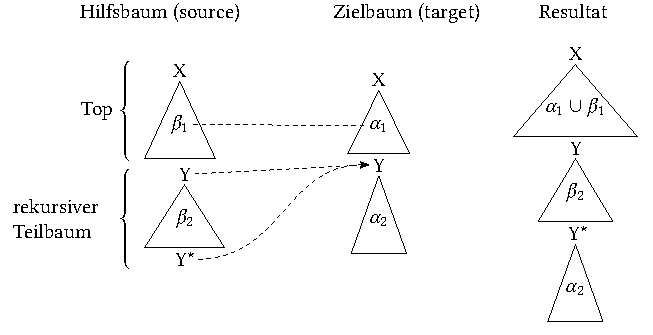
\includegraphics{graphics/abb611.pdf}
\caption{Segmentierte Adjunktion ohne Segmente (vgl.\ \citealt[Fig.~6.1]{Kulick:00})\label{fig-segmented-adj}}
\end{figure}

Entsprechend der Zweiteilung der Hilfsbäume ist nun auch deren Verknüpfung zweigeteilt: Der rekursive Teilbaum wird adjungiert, während der top"=Teilbaum mit dem Teilbaum oberhalb des Adjunktionsziels im Zielbaum {\it identifiziert}  wird ("`adjoin + identify"'). Die Identifizierung wird in Abbildung~\ref{fig-segmented-adj} im Resultat durch den Term $\alpha_1 \cup \beta_1$ angedeutet und kann tatsächlich als eingeschränkte Form der Graph-Unifikation verstanden werden \citep[93f]{Kulick:00}: In dem formalen Beispiel in Abbildung~\ref{fig-seg-formal} ist die Identifizierung der Knoten durch gestrichelte Linien ohne Pfeil angedeutet. Im resultierenden Baum stammt also das a-Blatt vom Zielbaum und das b-Blatt vom zweigeteilten Hilfsbaum. Mit dieser Verknüpfungsoperation gelingt es Kulick, die Teilstring-Beschränkung der ursprünglichen TAG-Adjunktion zu überwinden, d.\,h.\ sowohl der Zielbaum als auch der zweigeteilte Hilfsbaum können über die Identifikations-Operation beliebig viele diskontinuierliche Teilstrings beisteuern. 

\begin{figure}[t] 
\centering
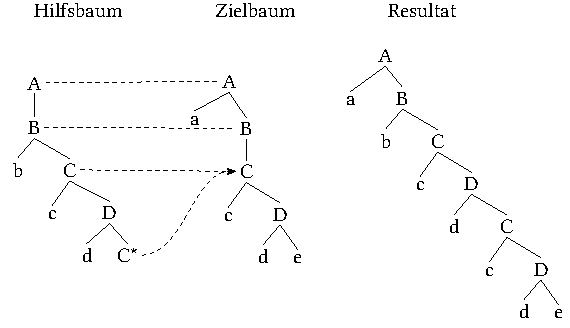
\includegraphics{graphics/abb612.pdf}
\caption{Formales Beispiel einer segmentierten Adjunktion (adjoin+identify, vgl.\ \citealt[(145), (146)]{Kulick:00})\label{fig-seg-formal}}
\end{figure} 
 
Die Frage, warum Kulick die Hilfsbäume teilt und die Identifikationsoperation so und nicht anders definiert, muss man wohl mit Blick auf die angestrebte Konstituentenstruktur beantworten. Kulick orientiert sich hierbei nämlich am CP-IP-Strukturparadigma der erweiterten Projektion\is{erweiterte Projektion}, das auch in Franks CETM implementiert wurde (siehe Abschnitt \ref{sec-tag-ling}). Demzufolge besitzen die von Kulick betrachteten Phänomene (Clitic Climbing, Kohärenz und Subjekt-Anhebung) zwar mehrere IPs (d.\,h.\ Verben), aber nur eine CP (d.\,h.\ nur ein Komplementierer oder nur ein finites Verb). Identifiziert werden also die CP-Teilbäume, während die IP-Teilbäume adjungieren. Dies beschränkt die Identifikation in der Praxis erheblich, da eine CP meist nur aus der Projektion von C besteht und damit die Menge der identifizierten Knoten nur C$'$ und CP umfasst. In der Praxis ist also Anzahl der diskontinuierlichen Teilstrings je Verknüpfung auf maximal 6 beschränkt, was jedoch ausreicht um Satz \ref{ex-schema2-2} adäquat zu analysieren, wie Abbildung~\ref{fig-seg-ling1} verdeutlicht:

\ex. {Dieses Buch} hat {den Kindern} niemand {zu geben} versucht.\label{ex-schema2-2} \\ 
(Wiederholung von \ref{ex-schema2}, S.~\pageref{ex-schema2}) 

\begin{figure}[p] 
\centering
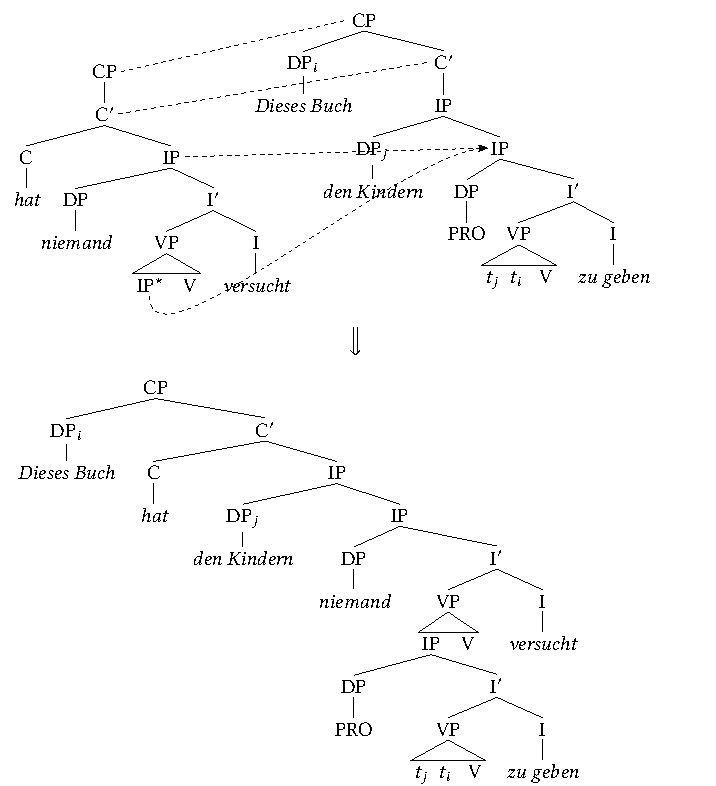
\includegraphics{graphics/abb613.pdf}
\caption{SegTAG-Analyse für Satz \ref{ex-schema2-2} (vgl.\ \citealt[(130) ,(131)]{Kulick:00})\label{fig-seg-ling1}}
\end{figure}

\noindent Allerdings gilt diese \isi{derivationelle Mächtigkeit} nur für Verbzweit-Sätze wie \ref{ex-schema2-2}. In der CP von Verbletzt-Sätzen besetzt der Komplementierer die Kopfposition in C und die SpecC-Position ist für Phrasen aus der IP unzugänglich. Die derivationelle Mächtigkeit reduziert sich dadurch wieder auf das Niveau von TAG. Das Verbletzt-Korrelat zu \ref{ex-schema2-2} in \ref{ex-seg-problem}  ist also weiterhin nicht adäquat modellierbar: 

\ex. da\ss \ des Verbrechens der Detektiv den Verdächtigen dem Klienten zu über-\linebreak führen versprochen hat\label{ex-seg-problem} \hfill (Wiederholung von \ref{ex-schema21}, S.~\pageref{ex-schema21})

Um dem abzuhelfen, verfügt SegTAG über eine weitere Fähigkeit, die bisher noch nicht erwähnt wurde. Sowohl der Zielbaum als auch der Hilfsbaum können {\it Segmente} inkorporieren, die elementarbaumübergreifend beliebig permutiert (d.\,h.\ verschachtelt) werden können. Elementarbaumbezogen müssen jedoch bestimmte Dominanzverhältnisse gewahrt bleiben. Im Hilfsbaum bilden Segmente diejenigen kleinsten rekursiven Teilstrukturen, die zwar mit dem Fu\ss knoten kategorie-identisch sind und ihn dominieren, diesen jedoch nicht enthalten.\footnote{Kulick nimmt auch für Initialbäume Segmente an, obwohl dies aus meiner Sicht nicht unbedingt nötig ist. Ihre Funktion ist in den Fällen, in denen der Hilfsbaum keine Segmente besitzt, alleine schon durch unterschiedliche Adjunktionsmöglichkeiten erfasst. Die restlichen Fälle sind mit den Segmenten der Hilfsbäume schon hinreichend erklärt.} In den linguistischen Beispielen sind die Segmente meist IP-Knoten, die wiederum einen IP-Knoten dominieren, und ihre nicht-IP-Kinder. In Abbildung~\ref{fig-seg-ling2} werden sie mittels gestrichelter Kanten angedeutet. Mit dieser Technik ist es auch bei Verbletzt-Sätzen möglich, in einer Verknüpfungsoperation beliebig viele Teilstrings zu erzeugen. Der zuvor problematische Satz \ref{ex-seg-problem} erhält somit die valenzadäquate Analyse in Abbildung~\ref{fig-seg-ling2}.      

\begin{figure}[p] 
\centering
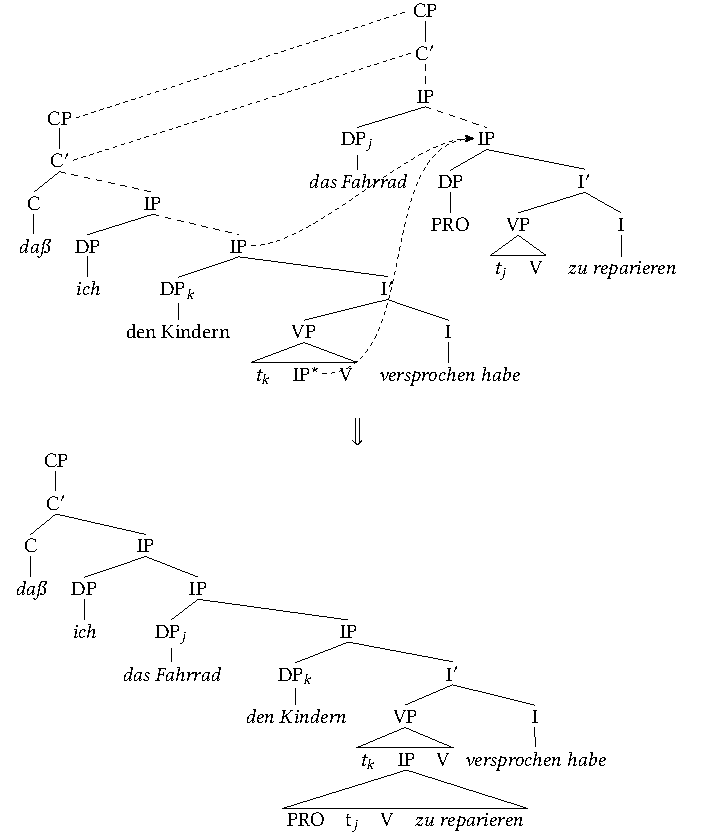
\includegraphics{graphics/abb614.pdf}
\caption{SegTAG-Analyse für den Satz \ref{ex-seg-problem} mit Segmenten (vgl.\ \citealt[(159), (160)]{Kulick:00})\label{fig-seg-ling2}}
\end{figure}

Die Permutierung der Segmente im Zuge einer Hilfsbaumverknüpfung bedeutet, dass die Adjunktion nicht der regulären TAG-Adjunktion entspricht. Dies ist auch daran ersichtlich, dass Kulick die Gestalt des Ableitungsbaums dahingehend ändern muss, dass die Segment-Sequenzen in die Knoten-Label kodiert sind. Darauf möchte ich aber hier nicht weiter eingehen. Eine wichtige Einschränkung der Segment-Permutierung kommt bei kohärenten Konstruktionen ins Spiel, die mehr als zwei Verben einschlie\ss en. Die Segmente aus nicht direkt verknüpften Bäumen können nämlich nicht beliebig permutieren, denn direkt verknüpfte Bäume bilden komplexe Segmente, die im weiteren Verlauf der Ableitung nicht mehr getrennt werden können (siehe \citealt[213ff]{Kulick:00}).

Diese Verklumpung der Segmente hat Folgen für die \isi{derivationelle Mächtigkeit} von SegTAG. Zwar ist SegTAG formal mächtiger als TAG, aber Kulick äu\ss ert die Vermutung, dass SegTAG nicht die Mächtigkeit besitzt, um die indizierte Sprache $\mathsf{SCR}^{ind}$\is{indizierte Scramblingsprache ($\mathsf{SCR}^{ind}$)} zu generieren \citep[215]{Kulick:00}.\footnote{Genauer gesagt vermutet Kulick, dass SegTAG die Ausdrucksstärke von LCFRS besitzt, und LCFRS kann $\mathsf{SCR}^{ind}$ nicht generieren (siehe Fußnote~\ref{fn-lcfrs}, S.\,\pageref{fn-lcfrs}).} Damit wäre SegTAG also nicht mächtig genug, um Scrambling in kohärenten Konstruktionen (zumindest kompetenzseitig) vollständig zu modellieren. Allerdings ermöglicht es SegTAG, kohärente Konstruktionen bis zu einem bestimmten Einbettungsgrad $k$ zu erfassen, d.\,h.\ die Teilmenge $k$-$\mathsf{SCR}^{ind}$ (siehe Abschnitt~\ref{sec-tag-grenzen-scram}):

\ex. $k$-$\mathsf{SCR}^{ind} = \{ \sigma(\mathit{NP}_1,\ldots,\mathit{NP}_k) V_1 \ldots V_k | k \geq 1$ und $\sigma$ ist eine Per"-mu"-tation$\}$

Die Elementarbäume werden mit steigendem Einbettungsgrad $k$ grö\ss er, denn es müssen dann leere Segmente installiert werden, um die Segment"=Verklumpungen wieder aufzubrechen. 

Da dies eine Einschränkung ist, der auch TL-MCTAG und SL-MCTAG unterworfen sind, liegt die Frage nahe, warum nicht statt SegTAG diese MCTAG-Varianten eingesetzt werden. Kulick argumentiert hier mit dem Hinweis auf Analysen für das Clitic-Climbing, die den MCTAG-Varianten wegen der Simultanitätsbedingungen verwehrt sind, in einem SegTAG-Ansatz aber zur Verfügung stehen \citep[53ff]{Kulick:00}. Durch die Identifikation und die Segment"=Permutation bei Adjunktion ist nämlich die Reihenfolge der Verknüpfung von der Reihenfolge der Konstituenten unabhängig.     

Als Fazit kann festgehalten werden, dass es Kulick zwar gelingt, eine TAG-Variante für die Erfassung von Kohärenzphänomenen zu entwickeln, die im Unterschied zu V-TAG und DTG eine Lokalitätsdomäne qua Elementarbaum verfügbar und die explizite Angabe von Barrieren in der Art der Integrity Constraints bzw.\ SICs überflüssig macht. Aber diese TAG-Variante muss dafür eine völlig neue Verknüpfungsoperation, die Identifikation, ins Leben rufen und die Adjunktion signifikant verändern. Wie sich diese Neuerungen auf die formalen Komplexitätseigenschaften auswirken, ist schwer abzusehen.
\is{Segmented TAG (SegTAG)|)}


\subsection{SN-MCTAG}\label{sec-snmctag}\is{TL-MCTAG with Shared Nodes (SN-MCTAG)|(}

Wir haben in Abschnitt~\ref{sec-tag-grenzen-scram} gesehen, dass TL-MCTAG (und auch SL-MCTAG) zwar eine im Vergleich zu TAG erhöhte derivationelle Mächtigkeit besitzt, dass diese jedoch nicht ausreicht, um die indizierte Scrambling-Sprache  $\mathsf{SCR}^{ind}$ korrekt zu erfassen. Eine Möglichkeit, dem abzuhelfen, besteht darin, eine nichtlokale MCTAG einzusetzen, wie dies etwa \cite{Rambow:94} mit V-TAG und \cite{Gerdes:04} mit TUG tun, wobei jedoch der Einsatz von zusätzlichen Mitteln notwendig wird, um die Lokalitätsdomäne zu reimplementieren. Einen anderen Weg geht deshalb \cite{Kallmeyer:05} mit SN-MCTAG (TL-MCTAG with shared nodes), indem sie die Lokalitätsdomäne von TL-MCTAG\is{Multi-Component TAG (MCTAG)!baumlokale (TL-MCTAG)} so erweitert, dass $\mathsf{SCR}^{ind}$\is{indizierte Scramblingsprache ($\mathsf{SCR}^{ind}$)} erfasst werden kann. 

Das zentrale Konzept dieser TL-MCTAG-Erweiterung ist das \textsc{Node Sharing}\is{Node Sharing}, dem die folgende Idee zugrunde liegt: Bei \isi{Adjunktion} und \isi{Substitution} wird der Zielknoten nicht vollständig durch einen Hilfsbaum bzw.\ Initialbaum ersetzt, d.\,h.\ er verschwindet nicht einfach, sondern er ist auch nach der Verknüpfung noch im Wurzelknoten und Fu\ss knoten des eingesetzten Hilfsbaums bzw.\ im Wurzelknoten des Initalbaums vorhanden. Der Wurzelknoten und Fu\ss knoten des eingesetzten Hilfsbaums wird also nach der Verknüpfung mit dem Zielbaum geteilt. Diese Idee findet man schon in der Merkmalsunifikation bei (FS)TAG\is{Feature-Structure-based TAG (FTAG)} (siehe Abschnitt~\ref{sec-tag-formalismus}): Bei Adjunktion wird der {\sc top}-Bereich des Zielknotens mit dem {\sc top}-Bereich des Hilfsbaumwurzelknotens und der {\sc bot}-Bereich des Zielknotens mit dem {\sc bot}-Bereich des Hilfsbaumfu\ss knotens unifiziert; bei Substitution unifizieren die {\sc top}-Bereiche des Zielknotens und des Wurzelknoten des eingesetzten Initialbaums. Wenn in SN-MCTAG also eine Baummenge $\Gamma$ mit einem Elementarbaum $\zeta$ verknüpft wird, dann können die Elementarbäume aus $\Gamma$ nicht nur direkt an einem Knoten von $\zeta$ adjungieren, sondern auch an geteilte Knoten von $\zeta$.

Sehen wir uns ein Beispiel an. Mit Node Sharing\is{Node Sharing} ist es möglich, den Satz \ref{ex-seg-problem2}, der mit einer TAG nicht adäquat modellierbar ist, mit den Elementarstrukturen in Abbildung~\ref{fig-snmctag-1} abzuleiten: 

\ex. dass ich das Fahrrad den Kindern zu reparieren versprochen habe \label{ex-seg-problem2}

Es handelt sich hierbei um eine Bewegungsanalyse\is{Bewegung}, d.\,h.\ die Baummengen bilden bewegte Nominalphrasen und ihre Spuren\is{Spur} ab. In einer Weirschen TL-MCTAG\is{Multi-Component TAG (MCTAG)!baumlokale (TL-MCTAG)} müsste solch ein NP-Spur-Paar direkt an den Zielbaum substituieren oder adjungieren, d.\,h.\ das Pronomen {\tt ich} und seine Spur {\tt t}$_{nom}$ müssten direkt mit dem Verb {\tt versprochen\_habe} verknüpft werden, wie beispielsweise bei der in Abbildung~\ref{fig-snmctag-2} dargestellten Derivation. Der Ableitungsbaum in Abbildung~\ref{fig-snmctag-1} zeigt jedoch, dass dies bei der Bewegungsanalyse nicht der Fall ist. Allerdings adjungiert {\tt ich} an einen geteilten Knoten von {\tt versprochen\_habe}, angezeigt durch eine gestrichelte Linie, was innerhalb der erweiterten Lokalität von SN-MCTAG liegt. Dasselbe gilt für die NP {\tt das\_Fahrrad} und seine Spur {\tt t}$_{acc}$.     

\begin{figure}[t]
\centering
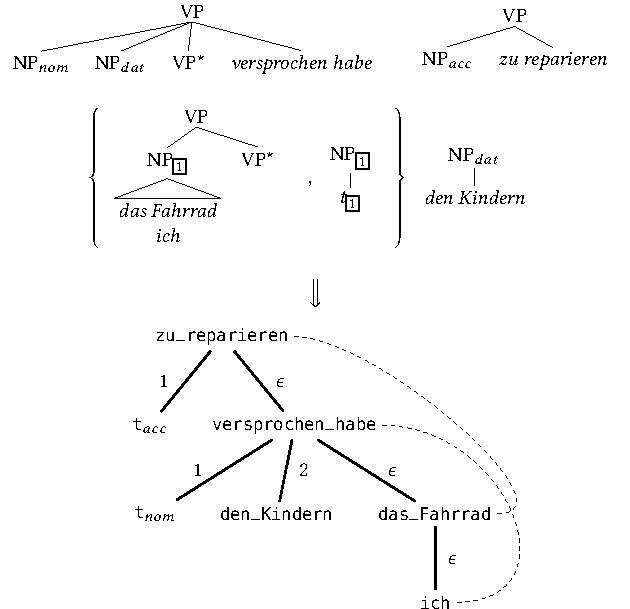
\includegraphics{graphics/abb615.pdf}
\caption{Elementarstrukturen und Ableitungsbaum einer SN-MCTAG-Bewegungs\-analyse von \ref{ex-seg-problem2}\label{fig-snmctag-1}}
\end{figure}

\begin{figure}[t]
\centering
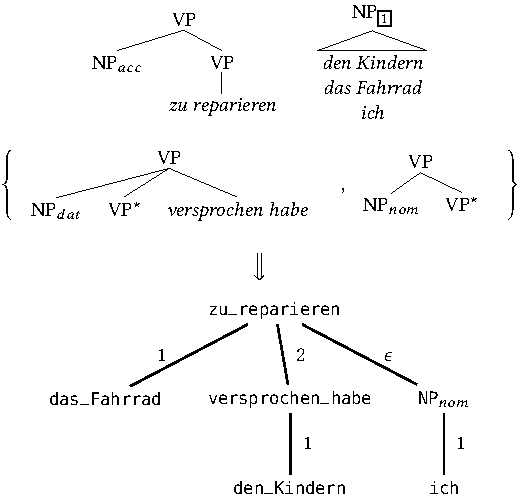
\includegraphics{graphics/abb616.pdf}
\caption{Elementarstrukturen und Ableitungsbaum einer TL-MCTAG-Analyse von \ref{ex-seg-problem2}\label{fig-snmctag-2}}
\end{figure}

Ob \isi{Node Sharing} besteht oder nicht, kann anhand der Dominanz-Pfade im \isi{Ableitungsbaum}festgestellt werden: Zwei Knoten $\gamma$, $\zeta$ in einem Ableitungsbaum $D$ stehen in einem Node-Sharing-Verhältnis, falls $\gamma$ von einem unmittelbaren Kind von $\zeta$ über eine Kette von Wurzeladjunktionen (mit Label $\epsilon$) dominiert wird. Bei der Benutzung einer Baummenge $\Gamma$ muss also erfüllt sein, dass es genau einen Knoten $\zeta$ in $D$ gibt, so dass für jedes $\gamma \in \Gamma$ gilt: Entweder $\zeta$ dominiert $\gamma$ unmittelbar, oder $\zeta$ dominiert $\gamma$ mittelbar und $\zeta$ und $\gamma$ stehen in einem Node-Sharing-Verhältnis. Eine formalere Darstellung des Node Sharings\is{Node Sharing} gibt es in Kapitel~\ref{sec-ttmctag} im Rahmen der Darstellung von \isi{TT-MCTAG}, bei der das Node Sharing ebenfalls eine zentrale Rolle spielt.\footnote{Ein wichtiger Unterschied ist allerdings, dass das \isi{Node Sharing} bei TT-MCTAG auf die Adjunktion beschränkt ist.} 

An den Beispielen in Abbildung~\ref{fig-snmctag-1} und \ref{fig-snmctag-2} wird deutlich, dass SN-MCTAG durch seine höhere derivationelle Mächtigkeit eine Bewegungsanalyse\is{Bewegung} für Satz \ref{ex-seg-problem2} zulässt, die mit TL-MCTAG nicht möglich ist: Die NP-Spur-Paare müssen bei TL-MCTAG direkt mit dem jeweils regierenden Verb verknüpft werden, wodurch die Einführung weiterer Diskontinuitäten ausgeschlossen ist. Was die Simulation von Bewegungsanalysen betrifft, gibt es zwischen TL-MCTAG und TAG also keinen Unterschied. Dagegen kann SN-MCTAG durch die um das Node Sharing erweiterte Lokalitätsdomäne auch die Scrambling-Sprache $\mathsf{SCR}^{ind}$\is{indizierte Scramblingsprache ($\mathsf{SCR}^{ind}$)} adäquat erfassen, die au\ss erhalb der absoluten derivationellen Mächtigkeit von TL-MCTAG liegt. Kallmeyer zeigt dies anhand der Elementarstrukturen in Abbildung~\ref{fig-snmctag-3}. Die Baummenge stellt hierbei die Koindizierung von \textit{NP} und \textit{V} sicher, während die Hilfsbäume der Baummenge über \isi{Node Sharing} am Start-Initialbaum adjungieren. Man muss jedoch beachten, dass in dieser Grammatik die \isi{Fu\ss knoten} keiner NA-Beschränkung\is{Adjunktionsbeschränkung} unterliegen dürfen, damit tatsächlich alle Permutationen von $\mathit{NP}_1, \ldots, \mathit{NP}_n$ abgeleitet werden können. Die \isi{Simultanitätsbedingung} macht dies notwendig. Allerdings ist es möglich, wie Abbildung~\ref{fig-snmctag-4} zeigt, eine entsprechende SN-MCTAG mit NA-Beschränkung\is{Adjunktionsbeschränkung} auf den Fu\ss knoten anzugeben. Dabei wird zunächst mittels der Elementarbäume eine Basisreihenfolge von NP-Slots erzeugt, die durch die NP-Spur-Baummenge beliebig permutiert werden können. 

\begin{figure}[t]
\centering
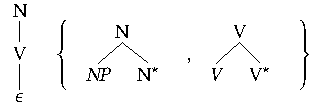
\includegraphics{graphics/abb617.pdf}
\caption{SN-MCTAG für die indizierte Sprache $\mathsf{SCR}^{ind}$ ohne NA-Beschränkung auf den Fu\ss knoten (vgl.\ \citealt[Figure~5]{Kallmeyer:05})\label{fig-snmctag-3}} 
\end{figure}

\begin{figure}[t]
\centering
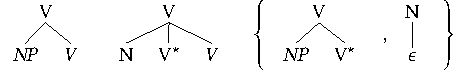
\includegraphics{graphics/abb618.pdf}
\caption{SN-MCTAG-Bewegungsanalyse für die indizierte Sprache $\mathsf{SCR}^{ind}$  mit NA-Beschränkung auf den Fu\ss knoten\label{fig-snmctag-4}}
\end{figure}

Was die Wohlgeformtheitsbedingungen\is{Wohlgeformtheitsprinzip} für SN-MCTAG-Elementarstrukturen im Rahmen einer Bewegungsanalyse betrifft, findet man in \cite{Kallmeyer:05} keine genaue Angaben. Man kann jedoch das Folgende annehmen: Für Elementarbäume in Baummengen mit nur einem Elementarbaum gelten die Wohlgeformtheitsbedingungen für TAG-Elementarbäume. Baummengen mit mehr Elementarbäumen dienen ausschlie\ss lich zur Modellierung von Bewegungen, d.\,h.\ sie enthalten einen Hilfsbaum für die bewegte Konstituente und einen Initialbaum für die \isi{Spur} in der Basisposition. Der Hilfsbaum der bewegten Konstitutente ist lexikalisiert und muss zusätzlich zu den durch das Valenzprinzip lizenzierten nicht-terminalen Blättern einen valenzfreien Fu\ss knoten besitzen.%\todo{OR: In V-Tag werden die Lokalitätsbeschrãnkungen verwendet, um z.B. Scrambling aus finiten Sätzen  oder Relativsätzen zu verhindern. Wie geht das in SN-MCTAG?} 

Die formalen Komplexitätseigenschaften von SN-MCTAG untersucht \cite{Kallmeyer:05} dagegen ausführlicher. Zunächst stellt sie fest, dass $\mathsf{SCR}^{ind}$\is{indizierte Scramblingsprache ($\mathsf{SCR}^{ind}$)} durch eine SN-MCTAG deriviert werden kann (siehe Abbildungen~\ref{fig-snmctag-3} und~\ref{fig-snmctag-4}). Da aber $\mathsf{SCR}^{ind}$ nicht von einer LCFRS erfasst werden kann \citep{Becker:Rambow:Niv:92} und LCFRS in der Literatur gerne zur Charakterisierung der MCS-Sprachen dient (\citealt{Kallmeyer:10b}), wird SN-MCTAG von Kallmeyer auf die Ausdrucksstärke von LCFRS\is{Linear Context-Free Rewriting Systems (LCFRS)} zurückgestutzt, indem sie zwei Änderungen vornimmt: Zum einen soll die Anzahl der Sekundärkanten ("`secondary edges"'), d.\,h.\ in unserer Notation die Anzahl der gestrichelten Kanten (vgl.\ Abbildung~\ref{fig-snmctag-1}), an einem Knoten im Ableitungsbaum beschränkt werden. Bisher kann ein Knoten im Ableitungsbaum beliebig viele Sekundärkanten besitzen. Erkennbar wird diese Eigenschaft etwa an der Grammatik für $\mathsf{SCR}^{ind}$ in Abbildung~\ref{fig-snmctag-3}: Die Elementarbäume beliebig vieler Baummengeninstanzen können an geteilte Knoten des Initialbaums adjungieren. Um dies zu verhindern, werden nur Ableitungen erlaubt, bei denen zumindest ein Elementarbaum einer Baummenge direkt am Zielbaum adjungiert oder substituiert. Dadurch ist die Anzahl der Sekundärkanten für einen Knoten $\gamma$ im Ableitungsbaum beschränkt durch die Anzahl der nicht-terminalen Knoten in $\gamma$ und die Grö\ss e der Baummengen. Kallmeyer nennt diese SN-MCTAG-Variante Restricted SN-MCTAG (RSN-MCTAG). Als RSN-MCTAG  kann die Grammatik in Abbildung~\ref{fig-snmctag-3} die Scrambling-Sprache $\mathsf{SCR}^{ind}$\is{indizierte Scramblingsprache ($\mathsf{SCR}^{ind}$)} nicht derivieren. Bei der Grammatik mit Bewegungsanalyse in Abbildung~\ref{fig-snmctag-4} bleibt dieses Potential allerdings auch im Rahmen von RSN-MCTAG erhalten. Entscheidend ist deshalb eine zweite Einschränkung: Eine RSN-MCTAG darf maximal eine festgelegte Stelligkeit $n$ besitzen, wobei die Stelligkeit von der Anzahl der Überkreuzungen von Sekundärkanten im Ableitungsbaum abhängt (siehe \citealt[212f]{Kallmeyer:05}). Nun ist auch die Derivation von $\mathsf{SCR}^{ind}$\is{indizierte Scramblingsprache ($\mathsf{SCR}^{ind}$)} durch die Grammatik in Abbildung~\ref{fig-snmctag-4} blockiert. Der Grad dieser Einschränkung kann jedoch beliebig hoch gesetzt werden, sodass eine beliebig gro\ss e, echte Teilmenge von $\mathsf{SCR}^{ind}$, nämlich $k$-$\mathsf{SCR}^{ind}$, erfasst werden kann und zumindest die im Sprachgebrauch auf"|tretenden Fälle abgedeckt sind. %\\

Zusammenfassend lässt sich also sagen, dass die Lokalitätserweiterung mittels \isi{Node Sharing} eine für Scrambling-Phänomene notwendige derivationelle Ausdrucksstärke zur Verfügung stellt. Im Unterschied zu V-TAG\is{Vector-MCTAG (V-TAG)} kann auf implizite Lokalitätsbeschränkungen qua Ableitungsbaum zurückgegriffen werden. Au\ss erdem zeichnet SN-MCTAG im Vergleich zu SegTAG\is{Segmented TAG (SegTAG)} ein höherer Grad der Formalisierung aus, was ein besseres Verständnis der formalen Komplexitätseigenschaften fördert. Ein Nachteil könnte jedoch sein, dass SN-MCTAG den Daten eine Bewegungsanalyse aufzwingt und dadurch anfällig für die Generierung unechter Ambiguität ist.\footnote{"`In order to avoid spurious ambiguities, we assume that whenever a derivation using the single elementary tree is possible, this is chosen."' \citep[203]{Kallmeyer:05}} Au\ss erdem erhält man bisweilen Bewegungsanalysen, die gar nicht benötigt werden (siehe \citealt[205]{Kallmeyer:05}). Wie wir gleich sehen  werden, gelingt es dagegen mit \isi{TT-MCTAG}, die Lokalitätserweiterung qua \isi{Node Sharing} zu nutzen, ohne eine Bewegungsanalyse mit den erwähnten Zugeständnissen implementieren zu müssen.
\is{TL-MCTAG with Shared Nodes (SN-MCTAG)|)}      


\subsection{TUG}

Etwas aus dem Rahmen fällt die \isi{Tree Unification Grammar (TUG)}, vorgestellt in \cite{Gerdes:04}. Es handelt sich hierbei um eine Art nicht-lokaler MCTAG\is{Multi-Component TAG (MCTAG)!nichtlokale (NL-MCTAG)}, der als Verknüpfungsoperation eine Form der Baumunifikation ("`unify"') nutzt. TUG dient allerdings primär zur Generierung wohlgeformter topologischer Strukturen. Die Beschränkung der Nicht-Lokalität scheint dagegen in den Aufgabenbereich anderer Grammatikmodule, des Dependenzmoduls und des Semantikmoduls, zu fallen. Leider sind Gerdes Angaben zu diesem Aspekt von TUG lückenhaft. Wie in V-TAG entsprechen die Baummengen Valenzrahmen, das hei\ss t, für die valenztheoretische Vollständigkeit wird bereits auf der topologischen Ebene gesorgt. Gerdes zeigt in seiner Arbeit die Mächtigkeit von TUG anhand von Daten mit partieller VP-Voranstellung, die auch in dieser Arbeit als zentrale Hürde bei der Modellierung kohärenter Konstruktionen wahrgenommen wird. Auf die Details seines Modellierungsansatzes möchte ich aber an dieser Stelle nicht weiter eingehen, gerade weil viele Details unklar sind. TUG wird uns jedoch im Zuge der Vorstellung des STUG-Modells in Kapitel~\ref{ch-ohne-valenz} wiederbegegnen, denn auch \isi{STUG} macht von der \isi{Baumunifikation} Gebrauch (allerdings nicht in der syntaktischen Domäne). 




\section{Zusammenfassung}

Die in diesem Abschnitt dargestellten TAG-Varianten sind prinzipiell dazu in der Lage, einen gro\ss en Teil der Diskontinuitätsphänomene\is{Diskontinuität} in kohärenten Konstruktionen\is{kohärente Konstruktion} valenztheoretisch adäquat zu modellieren. Es wurde in der Darstellung jedoch deutlich, dass jede dieser TAG-Varianten gewisse Nachteile mit sich bringt: V-TAG und DTG benötigen eine explizite Stipulation der Lokalitätsdomäne in den jeweiligen Elementarstrukturen. Bei SegTAG erfolgt die Stipulation der Lokalitätsdomäne zwar implizit, d.\,h.\ elementarbaumübergreifend, aber die formalen Eigenschaften der neuartigen Verknüpfungsoperationen, von denen SegTAG Gebrauch macht, bleiben gro\ss enteils im Dunkeln. SN-MCTAG ist zwar gründlich formalisiert und verfügt ebenfalls über eine implizit festgelegte Lokalitätsdomäne, funktioniert aber nur im Rahmen einer weitläufigen Bewegungsanalyse. 

Die Nachteile der bislang vorgeschlagenen TAG-Varianten definieren also den folgenden Anforderungskatalog für jede Neu- oder Weiterentwicklung: (i) Die Lokalitätsdomäne ist implizit festgelegt; (ii) das Verständnis für die Verknüpfungsoperationen und die Elementarstrukturen ist hinreichend klar, d.\,h.\ formalisiert; (iii) die Ausdrucksstärke und die Komplexitätseigenschaften befinden sich innerhalb des MCS-Bereichs und ermöglichen eine valenztheoretisch adäquate Modellierung kohärenter Konstruktionen; (iv) eine Bewegungsanalyse kann vermieden werden. Die Motivation zur Entwicklung von \isi{TT-MCTAG} ist es, genau diese Anforderungen zu erfüllen. 




















 
